\documentclass{article}

\usepackage[margin=1in]{geometry}
\usepackage{amsmath,amssymb,amsthm}
\usepackage{booktabs}
\usepackage{array}
\usepackage{longtable}
\usepackage{lipsum}
\usepackage{graphicx}
\usepackage{fancyhdr}
\usepackage[colorlinks=true, linkcolor=blue, urlcolor=blue, citecolor=blue]{hyperref}

\pagestyle{fancy}
\fancyhf{} % clear all header/footer fields
\fancyhead[L]{}
\fancyhead[R]{\thepage}
\renewcommand{\headrulewidth}{0.4pt}
\renewcommand{\footrulewidth}{0pt}

\title{Deep Learning}
\author{}

\begin{document}
\maketitle

\section{Metrics}

\subsection{Precision}
Precision, also known as Positive Predictive Value, measures the accuracy of the positive predictions made by the model.

\[
\text{Precision} = \frac{TP}{TP + FP}
\]

where:
- \( TP \) (True Positives) is the number of correct positive predictions.
- \( FP \) (False Positives) is the number of incorrect positive predictions.

\subsection{Recall}
Recall, also known as Sensitivity, True Positive Rate, or Hit Rate, measures the ability of the model to identify all relevant instances of the positive class.

\[
\text{Recall} = \frac{TP}{TP + FN}
\]

where:
- \( TP \) (True Positives) is the number of correct positive predictions.
- \( FN \) (False Negatives) is the number of incorrect negative predictions (actual positives that were not predicted as such).

\subsection{F1 Score}
The F1 Score is the harmonic mean of precision and recall.

\[
F1 \text{ Score} = 2 \times \frac{\text{Precision} \times \text{Recall}}{\text{Precision} + \text{Recall}}
\]

\subsection{Accuracy}
Accuracy measures the overall correctness of the model.

\[
\text{Accuracy} = \frac{TP + TN}{TP + TN + FP + FN}
\]

where:
- \( TN \) (True Negatives) is the number of correct negative predictions.

\subsection{Specificity}
Specificity, also known as True Negative Rate, measures the ability of the model to identify all negative instances.

\[
\text{Specificity} = \frac{TN}{TN + FP}
\]

\subsection{Negative Predictive Value (NPV)}
NPV measures the accuracy of negative predictions.

\[
\text{NPV} = \frac{TN}{TN + FN}
\]

\subsection{False Positive Rate (FPR)}
FPR measures the proportion of actual negatives that are incorrectly identified as positive.

\[
\text{FPR} = \frac{FP}{FP + TN}
\]

\subsection{False Negative Rate (FNR)}
FNR measures the proportion of actual positives that are incorrectly identified as negative.

\[
\text{FNR} = \frac{FN}{FN + TP}
\]

\subsection{Matthews Correlation Coefficient (MCC)}
MCC is a correlation coefficient between the observed and predicted binary classifications.

\[
\text{MCC} = \frac{(TP \times TN) - (FP \times FN)}{\sqrt{(TP + FP)(TP + FN)(TN + FP)(TN + FN)}}
\]

\subsection{Balanced Accuracy}
Balanced accuracy adjusts for imbalanced classes by taking the average of recall obtained on each class.

\[
\text{Balanced Accuracy} = \frac{\text{Sensitivity} + \text{Specificity}}{2}
\]





\subsection{Mean Absolute Error (MAE)}
\begin{equation}
L_{\text{MAE}}(\mathbf{y}, \hat{\mathbf{y}}) = \frac{1}{n} \sum_{i=1}^{n} |y_i - \hat{y}_i|
\end{equation}
\textbf{Derivative:}
\begin{equation}
\frac{\partial L_{\text{MAE}}}{\partial \hat{y}_i} = 
\begin{cases} 
\frac{1}{n} & \text{if } \hat{y}_i < y_i \\
-\frac{1}{n} & \text{if } \hat{y}_i > y_i 
\end{cases}
\end{equation}

\subsection{Mean Squared Error (MSE)}
\begin{equation}
L_{\text{MSE}}(\mathbf{y}, \hat{\mathbf{y}}) = \frac{1}{n} \sum_{i=1}^{n} (y_i - \hat{y}_i)^2
\end{equation}
\textbf{Derivative:}
\begin{equation}
\frac{\partial L_{\text{MSE}}}{\partial \hat{y}_i} = -\frac{2}{n} (y_i - \hat{y}_i)
\end{equation}

\subsection{Binary Cross-Entropy (BCE)}
\begin{equation}
L_{\text{BCE}}(\mathbf{y}, \hat{\mathbf{y}}) = -\frac{1}{n} \sum_{i=1}^{n} \left[ y_i \log(\hat{y}_i) + (1 - y_i) \log(1 - \hat{y}_i) \right]
\end{equation}
\textbf{Derivative:}
\begin{equation}
\frac{\partial L_{\text{BCE}}}{\partial \hat{y}_i} = -\frac{1}{n} \left( \frac{y_i}{\hat{y}_i} - \frac{1 - y_i}{1 - \hat{y}_i} \right)
\end{equation}

\subsection{Cross-Entropy (CE)}
\begin{equation}
L_{\text{CE}}(\mathbf{y}, \hat{\mathbf{y}}) = -\sum_{i=1}^{n} y_i \log(\hat{y}_i)
\end{equation}
\textbf{Derivative:}
\begin{equation}
\frac{\partial L_{\text{CE}}}{\partial \hat{y}_i} = -\frac{y_i}{\hat{y}_i}
\end{equation}

\subsection{Kullback-Leibler Divergence (KL Divergence)}
\begin{equation}
L_{\text{KL}}(\mathbf{p}, \mathbf{q}) = \sum_{i=1}^{n} p_i \log \left( \frac{p_i}{q_i} \right)
\end{equation}
\textbf{Derivative:}
\begin{equation}
\frac{\partial L_{\text{KL}}}{\partial q_i} = -\frac{p_i}{q_i}
\end{equation}

\subsection{Negative Log-Likelihood Loss (NLLLoss)}
\begin{equation}
L_{\text{NLL}}(\mathbf{y}, \hat{\mathbf{y}}) = -\sum_{i=1}^{n} \log(\hat{y}_{i, y_i})
\end{equation}
\textbf{Derivative:}
\begin{equation}
\frac{\partial L_{\text{NLL}}}{\partial \hat{y}_{i, y_i}} = -\frac{1}{\hat{y}_{i, y_i}}
\end{equation}

\subsection{Huber Loss}
\begin{equation}
L_{\text{Huber}}(\mathbf{y}, \hat{\mathbf{y}}) = 
\begin{cases} 
\frac{1}{2} (y_i - \hat{y}_i)^2 & \text{if } |y_i - \hat{y}_i| \leq \delta \\
\delta (|y_i - \hat{y}_i| - \frac{1}{2} \delta) & \text{otherwise}
\end{cases}
\end{equation}
\textbf{Derivative:}
\begin{equation}
\frac{\partial L_{\text{Huber}}}{\partial \hat{y}_i} = 
\begin{cases} 
-(y_i - \hat{y}_i) & \text{if } |y_i - \hat{y}_i| \leq \delta \\
-\delta \, \text{sign}(y_i - \hat{y}_i) & \text{otherwise}
\end{cases}
\end{equation}

\subsection{Hinge Loss}
\begin{equation}
L_{\text{Hinge}}(\mathbf{y}, \hat{\mathbf{y}}) = \sum_{i=1}^{n} \max(0, 1 - y_i \hat{y}_i)
\end{equation}
\textbf{Derivative:}
\begin{equation}
\frac{\partial L_{\text{Hinge}}}{\partial \hat{y}_i} = 
\begin{cases} 
0 & \text{if } y_i \hat{y}_i \geq 1 \\
-y_i & \text{if } y_i \hat{y}_i < 1
\end{cases}
\end{equation}








\section{Variations of ReLU}

\subsection{ReLU (Rectified Linear Unit)}
The ReLU function is defined as:
\begin{equation}
\text{ReLU}(x) = \max(0, x)
\end{equation}
Its first-order derivative is:
\begin{equation}
\text{ReLU}'(x) = 
\begin{cases} 
0 & \text{if } x \leq 0 \\
1 & \text{if } x > 0 
\end{cases}
\end{equation}

\subsection{Leaky ReLU}
The Leaky ReLU function introduces a small slope for negative values:
\begin{equation}
\text{LeakyReLU}(x) = 
\begin{cases} 
\alpha x & \text{if } x \leq 0 \\
x & \text{if } x > 0 
\end{cases}
\end{equation}
Its first-order derivative is:
\begin{equation}
\text{LeakyReLU}'(x) = 
\begin{cases} 
\alpha & \text{if } x \leq 0 \\
1 & \text{if } x > 0 
\end{cases}
\end{equation}
where \( \alpha \) is a small constant.

\subsection{Parametric ReLU (PReLU)}
The PReLU function is similar to Leaky ReLU but allows the slope to be learned:
\begin{equation}
\text{PReLU}(x) = 
\begin{cases} 
a x & \text{if } x \leq 0 \\
x & \text{if } x > 0 
\end{cases}
\end{equation}
Its first-order derivative is:
\begin{equation}
\text{PReLU}'(x) = 
\begin{cases} 
a & \text{if } x \leq 0 \\
1 & \text{if } x > 0 
\end{cases}
\end{equation}
where \( a \) is a parameter learned during training.

\subsection{ELU (Exponential Linear Unit)}
The ELU function is defined as:
\begin{equation}
\text{ELU}(x) = 
\begin{cases} 
\alpha (e^x - 1) & \text{if } x \leq 0 \\
x & \text{if } x > 0 
\end{cases}
\end{equation}
Its first-order derivative is:
\begin{equation}
\text{ELU}'(x) = 
\begin{cases} 
\alpha e^x & \text{if } x \leq 0 \\
1 & \text{if } x > 0 
\end{cases}
\end{equation}
where \( \alpha \) is a positive constant.

\subsection{RReLU (Randomized Leaky ReLU)}
The RReLU function introduces a randomized slope for negative values during training:
\begin{equation}
\text{RReLU}(x) = 
\begin{cases} 
\alpha x & \text{if } x \leq 0 \\
x & \text{if } x > 0 
\end{cases}
\end{equation}
Its first-order derivative is:
\begin{equation}
\text{RReLU}'(x) = 
\begin{cases} 
\alpha & \text{if } x \leq 0 \\
1 & \text{if } x > 0 
\end{cases}
\end{equation}
where \( \alpha \) is a random value in a given range during training and a fixed value during testing.

\subsection{SELU (Scaled Exponential Linear Unit)}
The SELU function is defined as:
\begin{equation}
\text{SELU}(x) = \lambda 
\begin{cases} 
\alpha (e^x - 1) & \text{if } x \leq 0 \\
x & \text{if } x > 0 
\end{cases}
\end{equation}
Its first-order derivative is:
\begin{equation}
\text{SELU}'(x) = \lambda
\begin{cases} 
\alpha e^x & \text{if } x \leq 0 \\
1 & \text{if } x > 0 
\end{cases}
\end{equation}
where \( \alpha \) and \( \lambda \) are fixed parameters.

\subsection{GELU (Gaussian Error Linear Unit)}
The GELU function is defined as:
\begin{equation}
\text{GELU}(x) = x \Phi(x)
\end{equation}
where \( \Phi(x) \) is the cumulative distribution function of the standard normal distribution. A common approximation is:
\begin{equation}
\text{GELU}(x) \approx 0.5 x \left(1 + \tanh\left(\sqrt{\frac{2}{\pi}} (x + 0.044715 x^3)\right)\right)
\end{equation}
Its first-order derivative is more complex and often approximated in practice.

\subsection{SiLU (Sigmoid Linear Unit or Swish)}
The SiLU function is defined as:
\begin{equation}
\text{SiLU}(x) = x \sigma(x)
\end{equation}
where \( \sigma(x) \) is the sigmoid function. Its first-order derivative is:
\begin{equation}
\text{SiLU}'(x) = \sigma(x) + x \sigma(x) (1 - \sigma(x))
\end{equation}
where \( \sigma(x) = \frac{1}{1 + e^{-x}} \).

\subsection{GLU (Gated Linear Unit)}
The GLU function is defined as:
\begin{equation}
\text{GLU}(a, b) = a \otimes \sigma(b)
\end{equation}
where \( a \) and \( b \) are inputs, \( \sigma \) is the sigmoid function, and \( \otimes \) denotes element-wise multiplication. The first-order derivative is more complex and depends on the context in which it is used.


\section{Optimizers}

\subsection{Momentum}
Momentum helps accelerate gradient vectors in the right directions, thus leading to faster converging.
\begin{equation}
v_t = \beta v_{t-1} + \eta \nabla L(\theta_t)
\end{equation}
\begin{equation}
\theta_{t+1} = \theta_t - v_t
\end{equation}
where:
\begin{itemize}
    \item $v_t$ is the velocity at time step $t$.
    \item $\beta$ is the momentum coefficient.
    \item $\eta$ is the learning rate.
    \item $\nabla L(\theta_t)$ is the gradient of the loss function at time step $t$.
    \item $\theta_t$ are the parameters at time step $t$.
\end{itemize}

\subsection{Nesterov Momentum}
Nesterov Momentum is a variant of momentum that anticipates the gradient and uses the gradient at the approximated future position.
\begin{equation}
v_t = \beta v_{t-1} + \eta \nabla L(\theta_t - \beta v_{t-1})
\end{equation}
\begin{equation}
\theta_{t+1} = \theta_t - v_t
\end{equation}
where:
\begin{itemize}
    \item $v_t$ is the velocity at time step $t$.
    \item $\beta$ is the momentum coefficient.
    \item $\eta$ is the learning rate.
    \item $\nabla L(\theta_t - \beta v_{t-1})$ is the gradient of the loss function at the anticipated future position.
    \item $\theta_t$ are the parameters at time step $t$.
\end{itemize}

\subsection{Polyak's Momentum}
Polyak's Momentum method uses the concept of momentum to stabilize convergence and avoid oscillations.
\begin{equation}
v_t = \beta v_{t-1} + \eta \nabla L(\theta_t)
\end{equation}
\begin{equation}
\theta_{t+1} = \theta_t - (1 + \beta) v_t
\end{equation}
where:
\begin{itemize}
    \item $v_t$ is the velocity at time step $t$.
    \item $\beta$ is the momentum coefficient.
    \item $\eta$ is the learning rate.
    \item $\nabla L(\theta_t)$ is the gradient of the loss function at time step $t$.
    \item $\theta_t$ are the parameters at time step $t$.
\end{itemize}

\subsection{RMSProp (Root Mean Square Propagation)}
RMSProp divides the learning rate by an exponentially decaying average of squared gradients.
\begin{equation}
v_t = \beta v_{t-1} + (1 - \beta) (\nabla L(\theta_t))^2
\end{equation}
\begin{equation}
\theta_{t+1} = \theta_t - \frac{\eta}{\sqrt{v_t} + \epsilon} \nabla L(\theta_t)
\end{equation}
where:
\begin{itemize}
    \item $v_t$ is the moving average of squared gradients at time step $t$.
    \item $\beta$ is the decay rate.
    \item $\eta$ is the learning rate.
    \item $\nabla L(\theta_t)$ is the gradient of the loss function at time step $t$.
    \item $\epsilon$ is a small constant for numerical stability.
    \item $\theta_t$ are the parameters at time step $t$.
\end{itemize}







\section{Adam (Adaptive Moment Estimation)}

Adam is an adaptive learning rate optimization algorithm that combines the advantages of two other popular methods: AdaGrad and RMSProp. It uses estimates of the first and second moments of the gradients to adapt the learning rate for each parameter.

\subsection{First Moment Estimate}
\begin{equation}
m_t = \beta_1 m_{t-1} + (1 - \beta_1) g_t
\end{equation}
where:
\begin{itemize}
    \item $m_t$ is the first moment estimate (mean of gradients).
    \item $\beta_1$ is the exponential decay rate for the first moment estimate.
    \item $g_t$ is the gradient at time step $t$.
\end{itemize}

\subsection{Second Moment Estimate}
\begin{equation}
v_t = \beta_2 v_{t-1} + (1 - \beta_2) g_t^2
\end{equation}
where:
\begin{itemize}
    \item $v_t$ is the second moment estimate (uncentered variance of gradients).
    \item $\beta_2$ is the exponential decay rate for the second moment estimate.
\end{itemize}

\subsection{Bias Correction}
\begin{equation}
\hat{m}_t = \frac{m_t}{1 - \beta_1^t}
\end{equation}
\begin{equation}
\hat{v}_t = \frac{v_t}{1 - \beta_2^t}
\end{equation}
where:
\begin{itemize}
    \item $\hat{m}_t$ is the bias-corrected first moment estimate.
    \item $\hat{v}_t$ is the bias-corrected second moment estimate.
\end{itemize}

\subsection{Parameter Update}
\begin{equation}
\theta_{t+1} = \theta_t - \eta \frac{\hat{m}_t}{\sqrt{\hat{v}_t} + \epsilon}
\end{equation}
where:
\begin{itemize}
    \item $\theta_{t+1}$ is the updated parameter.
    \item $\theta_t$ is the current parameter.
    \item $\eta$ is the learning rate.
    \item $\epsilon$ is a small constant added for numerical stability.
\end{itemize}




\section{Variants of Adam}

\subsection{AdamW (Adam with Weight Decay)}
AdamW decouples weight decay from the gradient update, improving regularization and generalization.
\begin{equation}
m_t = \beta_1 m_{t-1} + (1 - \beta_1) g_t
\end{equation}
\begin{equation}
v_t = \beta_2 v_{t-1} + (1 - \beta_2) g_t^2
\end{equation}
\begin{equation}
\hat{m}_t = \frac{m_t}{1 - \beta_1^t}
\end{equation}
\begin{equation}
\hat{v}_t = \frac{v_t}{1 - \beta_2^t}
\end{equation}
\begin{equation}
\theta_{t+1} = \theta_t - \eta \left( \frac{\hat{m}_t}{\sqrt{\hat{v}_t} + \epsilon} + \lambda \theta_t \right)
\end{equation}
where:
\begin{itemize}
    \item $\lambda$ is the weight decay coefficient.
\end{itemize}

\subsection{AdaMax}
AdaMax is a variant of Adam based on the infinity norm.
\begin{equation}
m_t = \beta_1 m_{t-1} + (1 - \beta_1) g_t
\end{equation}
\begin{equation}
u_t = \max(\beta_2 u_{t-1}, |g_t|)
\end{equation}
\begin{equation}
\hat{m}_t = \frac{m_t}{1 - \beta_1^t}
\end{equation}
\begin{equation}
\theta_{t+1} = \theta_t - \frac{\eta}{u_t + \epsilon} \hat{m}_t
\end{equation}

\subsection{NAdam (Nesterov-accelerated Adaptive Moment Estimation)}
NAdam incorporates Nesterov momentum into Adam.
\begin{equation}
m_t = \beta_1 m_{t-1} + (1 - \beta_1) g_t
\end{equation}
\begin{equation}
v_t = \beta_2 v_{t-1} + (1 - \beta_2) g_t^2
\end{equation}
\begin{equation}
\hat{m}_t = \frac{m_t}{1 - \beta_1^t}
\end{equation}
\begin{equation}
\hat{v}_t = \frac{v_t}{1 - \beta_2^t}
\end{equation}
\begin{equation}
\theta_{t+1} = \theta_t - \eta \left( \frac{\beta_1 \hat{m}_t + (1 - \beta_1) g_t}{\sqrt{\hat{v}_t} + \epsilon} \right)
\end{equation}

\subsection{RAdam (Rectified Adam)}
RAdam introduces a rectification term to the Adam optimizer.
\begin{equation}
m_t = \beta_1 m_{t-1} + (1 - \beta_1) g_t
\end{equation}
\begin{equation}
v_t = \beta_2 v_{t-1} + (1 - \beta_2) g_t^2
\end{equation}
\begin{equation}
\hat{m}_t = \frac{m_t}{1 - \beta_1^t}
\end{equation}
\begin{equation}
\hat{v}_t = \frac{v_t}{1 - \beta_2^t}
\end{equation}
\begin{equation}
\rho_t = \rho_{\infty} - \frac{2t\beta_2^t}{1 - \beta_2^t}
\end{equation}
\begin{equation}
r_t = \sqrt{\frac{(\rho_t - 4)(\rho_t - 2)\rho_{\infty}}{(\rho_{\infty} - 4)(\rho_{\infty} - 2)\rho_t}}
\end{equation}
\begin{equation}
\theta_{t+1} = \theta_t - \eta r_t \frac{\hat{m}_t}{\sqrt{\hat{v}_t} + \epsilon}
\end{equation}
or, if \( \rho_t \leq 4 \):
\begin{equation}
\theta_{t+1} = \theta_t - \eta \frac{\hat{m}_t}{\sqrt{\hat{v}_t} + \epsilon}
\end{equation}
where:
\begin{itemize}
    \item $\rho_{\infty} = \frac{2}{1 - \beta_2} - 1$
\end{itemize}











\section{Xavier Initialization}

Xavier Initialization, also known as Glorot Initialization, aims to keep the scale of the gradients roughly the same in all layers, which is particularly useful for activation functions like sigmoid and Tanh.

This ensures the variance of the output is the same as the input, assuming a Gaussian distribution with:
\begin{itemize}
    \item Mean: $\mathbb{E}[X] = 0$, $\mathbb{E}[W] = 0$
    \item Variance: Remember that $\mathbb{E}[X^2] = \text{Var}[X] + \mathbb{E}[X]^2$ and if $X, Y$ are independent:
    \begin{equation}
    \text{Var}[XY] = \mathbb{E}[X^2 Y^2] - \mathbb{E}[XY]^2
    \end{equation}
    \begin{equation}
    \mathbb{E}[XY] = \mathbb{E}[X]\mathbb{E}[Y]
    \end{equation}
\end{itemize}

Therefore,
\begin{equation}
\text{Var}(s) = \text{Var} \left( \sum_{i}^n w_i x_i \right) = \sum_{i}^n \text{Var} (w_i x_i)
\end{equation}
\begin{equation}
= \sum_{i}^n \left[ \mathbb{E} (w_i) \right]^2 \text{Var} (x_i) + \left[ \mathbb{E} (x_i) \right]^2 \text{Var} (w_i) + \text{Var} (x_i) \text{Var} (w_i)
\end{equation}
\begin{equation}
= \sum_{i}^n \text{Var} (x_i) \text{Var} (w_i) = n (\text{Var} (w) \text{Var} (x))
\end{equation}

We want to ensure that the variance of the output $s = xw$ is the same as the input: $\text{Var}(s) = \text{Var}(x)$.

\begin{equation}
\text{Var} (w) = n (\text{Var} (w) \text{Var} (x)) \rightarrow \text{Var} (w) = \frac{1}{n}
\end{equation}

Note that $n$ is the number of input neurons for the layer of weights you want to initialize. This $n$ is not the number $N$ of input data $X \in \mathbb{R}^{N \times D}$, but $n = D$.
















\section{Regularization terms}

The L2-regularization term is added to the loss function to penalize large weights. For a given loss function \( L \) and weights \( W \), the regularized loss function \( L_{\text{reg}} \) can be written as:

\[
L_{\text{reg}} = L + \frac{\lambda}{2} \|W\|_2^2
\]

where \( \frac{\lambda}{2} \|W\|_2^2 \) is the L2-regularization term and \( \|W\|_2^2 = \sum_{i} W_i^2 \) is the squared Euclidean norm of the weights.

\section*{Gradient Descent Update Rule with L2-Regularization}

In gradient descent, the weights are updated iteratively using the gradient of the loss function. The update rule for the weights \( W \) at iteration \( t \) without regularization is:

\[
W^{(t+1)} = W^{(t)} - \eta \nabla_W L
\]

When we include L2-regularization, the gradient of the regularized loss function \( L_{\text{reg}} \) with respect to the weights \( W \) becomes:

\[
\nabla_W L_{\text{reg}} = \nabla_W L + \lambda W
\]

Therefore, the update rule with L2-regularization is:

\[
W^{(t+1)} = W^{(t)} - \eta \left( \nabla_W L + \lambda W \right)
\]

\section*{Interpreting the Update Rule}

Let's rewrite the update rule to separate the effect of L2-regularization:

\[
W^{(t+1)} = W^{(t)} - \eta \nabla_W L - \eta \lambda W^{(t)}
\]

Rearrange this to highlight the weight decay effect:

\[
W^{(t+1)} = W^{(t)} \left( 1 - \eta \lambda \right) - \eta \nabla_W L
\]

Here, we can see that the term \( W^{(t)} \left( 1 - \eta \lambda \right) \) represents a multiplicative factor that scales the weights down. This multiplicative factor \( 1 - \eta \lambda \) is always less than 1 if \( \eta \lambda > 0 \), causing the weights to decay at each iteration. This is why L2-regularization is referred to as "weight decay."

\section*{Summary}

The term "weight decay" comes from the effect of L2-regularization on the weights during the gradient descent update. The update rule with L2-regularization:

\[
W^{(t+1)} = W^{(t)} \left( 1 - \eta \lambda \right) - \eta \nabla_W L
\]

shows that the weights are scaled down by a factor of \( 1 - \eta \lambda \) at each iteration, effectively decaying the weights over time. This regularization helps to prevent overfitting by encouraging smaller weights, leading to simpler and more generalizable models.

\section*{Other Regularization terms}

\subsection*{1. Elastic Net Regularization}
\[
\text{Loss} = \text{Primary Loss} + \lambda_1 \sum_{i=1}^{n} |w_i| + \frac{1}{2} \lambda_2 \sum_{i=1}^{n} w_i^2
\]
\[
w \leftarrow w - \eta \left( \frac{\partial \text{Primary Loss}}{\partial w} + \lambda_1 \text{sign}(w) + \lambda_2 w \right)
\]

\subsection*{2. Tikhonov Regularization (L2 Regularization)}
\[
\text{Loss} = \text{Primary Loss} + \frac{1}{2} \lambda \sum_{i=1}^{n} w_i^2
\]
\[
w \leftarrow w - \eta \left( \frac{\partial \text{Primary Loss}}{\partial w} + \lambda w \right)
\]

\subsection*{3. Spectral Norm Regularization}
\[
\text{Loss} = \text{Primary Loss} + \lambda \|W\|_2
\]
\[
w \leftarrow w - \eta \left( \frac{\partial \text{Primary Loss}}{\partial w} + \lambda \frac{\partial \|W\|_2}{\partial w} \right)
\]

\subsection*{4. Orthogonality Regularization}
\[
\text{Loss} = \text{Primary Loss} + \lambda \|W^T W - I\|_F^2
\]
\[
w \leftarrow w - \eta \left( \frac{\partial \text{Primary Loss}}{\partial w} + \lambda \frac{\partial \|W^T W - I\|_F^2}{\partial w} \right)
\]

\subsection*{5. Max-Norm Regularization}
\[
\text{Loss} = \text{Primary Loss} + \lambda \sum_{i=1}^{n} \max(0, \|w_i\|_2 - c)
\]
\[
w \leftarrow w - \eta \left( \frac{\partial \text{Primary Loss}}{\partial w} \right)
\]
After updating, project the weights onto the \(L_2\) ball of radius \(c\):
\[
w_i \leftarrow \frac{w_i}{\max(1, \|w_i\|_2 / c)}
\]













\section{Batch Normalization}

Given a fully connected layer with an output shape of $8 \times 16$, followed by a batch normalization layer, the operation can be expressed as $y = \text{BN}(x) = \gamma \ast x_{\text{norm}} + \beta$.

\subsection*{(a) Dimensions of the Parameters $\gamma$ and $\beta$}

\begin{itemize}
    \item Since batch normalization is applied per feature (i.e., per column in the output of the fully connected layer), the parameters $\gamma$ and $\beta$ will each have dimensions equal to the number of features.
    \item For the given output shape $8 \times 16$:
    \begin{itemize}
        \item $\gamma$ and $\beta$ will each have a dimension of $16$.
    \end{itemize}
    \item Therefore:
    \begin{itemize}
        \item $\gamma$ has shape $(16,)$
        \item $\beta$ has shape $(16,)$
    \end{itemize}
\end{itemize}

\subsection*{(b) Derivation of the Gradients of $\gamma$ and $\beta$}

To derive the gradients of the loss $L$ with respect to $\gamma$ and $\beta$, we start by defining the batch normalization operation more formally.

Let:
\begin{itemize}
    \item $x \in \mathbb{R}^{8 \times 16}$ be the input to the batch normalization layer.
    \item $\mu = \frac{1}{N} \sum_{i=1}^{N} x_i$ be the mean of the input $x$.
    \item $\sigma^2 = \frac{1}{N} \sum_{i=1}^{N} (x_i - \mu)^2$ be the variance of the input $x$.
    \item $x_{\text{norm}} = \frac{x - \mu}{\sqrt{\sigma^2 + \epsilon}}$ be the normalized input.
    \item $y = \gamma \ast x_{\text{norm}} + \beta$ be the output of the batch normalization layer.
\end{itemize}

We need to find the partial derivatives $\frac{\partial L}{\partial \gamma}$ and $\frac{\partial L}{\partial \beta}$.

\subsubsection*{1. Gradient with respect to $\beta$:}

The gradient of the loss $L$ with respect to $\beta$ is the sum of the gradients of the loss with respect to each output $y_i$:
\[
\frac{\partial L}{\partial \beta_j} = \sum_{i=1}^{N} \frac{\partial L}{\partial y_{ij}} \cdot \frac{\partial y_{ij}}{\partial \beta_j}
\]

Since $\frac{\partial y_{ij}}{\partial \beta_j} = 1$, we get:
\[
\frac{\partial L}{\partial \beta_j} = \sum_{i=1}^{N} \frac{\partial L}{\partial y_{ij}}
\]

\subsubsection*{2. Gradient with respect to $\gamma$:}

The gradient of the loss $L$ with respect to $\gamma$ is the sum of the gradients of the loss with respect to each output $y_i$ multiplied by the normalized input $x_{\text{norm}}$:
\[
\frac{\partial L}{\partial \gamma_j} = \sum_{i=1}^{N} \frac{\partial L}{\partial y_{ij}} \cdot \frac{\partial y_{ij}}{\partial \gamma_j}
\]

Since $\frac{\partial y_{ij}}{\partial \gamma_j} = x_{\text{norm}_{ij}}$, we get:
\[
\frac{\partial L}{\partial \gamma_j} = \sum_{i=1}^{N} \frac{\partial L}{\partial y_{ij}} \cdot x_{\text{norm}_{ij}}
\]

\subsection*{(c) Using NumPy to Calculate Gradients}

Let's assume:
\begin{itemize}
    \item \texttt{dL\_dy} is the gradient of the loss $L$ with respect to the output $y$, with shape $(8, 16)$.
    \item \texttt{x\_norm} is the normalized input, with shape $(8, 16)$.
\end{itemize}

Using NumPy, we can calculate the gradients as follows:

\begin{verbatim}
import numpy as np

# Assuming dL_dy and x_norm are given as NumPy arrays
dL_dy = np.random.randn(8, 16)  # Example gradient of the loss with respect to y
x_norm = np.random.randn(8, 16)  # Example normalized input

# Gradient with respect to beta
dL_dbeta = np.sum(dL_dy, axis=0)

# Gradient with respect to gamma
dL_dgamma = np.sum(dL_dy * x_norm, axis=0)

# Print the results
print("Gradient with respect to beta:", dL_dbeta)
print("Gradient with respect to gamma:", dL_dgamma)
\end{verbatim}

In this code:
\begin{itemize}
    \item \texttt{np.sum(dL\_dy, axis=0)} computes the sum of \texttt{dL\_dy} along the batch dimension (axis 0) to get $\frac{\partial L}{\partial \beta}$.
    \item \texttt{np.sum(dL\_dy * x\_norm, axis=0)} computes the sum of the element-wise product of \texttt{dL\_dy} and \texttt{x\_norm} along the batch dimension to get $\frac{\partial L}{\partial \gamma}$.
\end{itemize}

This gives us the gradients of the loss with respect to the parameters $\gamma$ and $\beta$.













\subsection{Batch Normalization Backpropagation in CNNs}

Batch Normalization (BN) is a technique to normalize the inputs of each layer, improving training speed and stability. Here, we demonstrate the backpropagation through BN in CNNs using a small example.

\subsection{Forward Pass}

Consider a mini-batch of inputs \( \mathbf{X} = \{ \mathbf{x}_1, \mathbf{x}_2, \dots, \mathbf{x}_m \} \) with \( \mathbf{x}_i \in \mathbb{R}^D \). The steps of the forward pass through BN are:

\begin{itemize}
    \item Compute the mini-batch mean:
    \begin{equation}
    \mu_B = \frac{1}{m} \sum_{i=1}^{m} \mathbf{x}_i
    \end{equation}

    \item Compute the mini-batch variance:
    \begin{equation}
    \sigma_B^2 = \frac{1}{m} \sum_{i=1}^{m} (\mathbf{x}_i - \mu_B)^2
    \end{equation}

    \item Normalize the batch:
    \begin{equation}
    \hat{\mathbf{x}}_i = \frac{\mathbf{x}_i - \mu_B}{\sqrt{\sigma_B^2 + \epsilon}}
    \end{equation}

    \item Scale and shift:
    \begin{equation}
    \mathbf{y}_i = \gamma \hat{\mathbf{x}}_i + \beta
    \end{equation}
\end{itemize}

\subsection{Backward Pass}

Given the gradient of the loss \( L \) with respect to the output \( \frac{\partial L}{\partial \mathbf{y}_i} \), we want to compute the gradients with respect to \( \mathbf{x}_i \), \( \gamma \), and \( \beta \).

\begin{itemize}
    \item Gradient with respect to \( \beta \):
    \begin{equation}
    \frac{\partial L}{\partial \beta} = \sum_{i=1}^{m} \frac{\partial L}{\partial \mathbf{y}_i}
    \end{equation}

    \item Gradient with respect to \( \gamma \):
    \begin{equation}
    \frac{\partial L}{\partial \gamma} = \sum_{i=1}^{m} \frac{\partial L}{\partial \mathbf{y}_i} \cdot \hat{\mathbf{x}}_i
    \end{equation}

    \item Gradient with respect to \( \hat{\mathbf{x}}_i \):
    \begin{equation}
    \frac{\partial L}{\partial \hat{\mathbf{x}}_i} = \frac{\partial L}{\partial \mathbf{y}_i} \cdot \gamma
    \end{equation}

    \item Gradient with respect to \( \sigma_B^2 \):
    \begin{equation}
    \frac{\partial L}{\partial \sigma_B^2} = \sum_{i=1}^{m} \frac{\partial L}{\partial \hat{\mathbf{x}}_i} \cdot (\mathbf{x}_i - \mu_B) \cdot -\frac{1}{2} (\sigma_B^2 + \epsilon)^{-3/2}
    \end{equation}

    \item Gradient with respect to \( \mu_B \):
    \begin{equation}
    \frac{\partial L}{\partial \mu_B} = \sum_{i=1}^{m} \left( \frac{\partial L}{\partial \hat{\mathbf{x}}_i} \cdot -\frac{1}{\sqrt{\sigma_B^2 + \epsilon}} \right) + \frac{\partial L}{\partial \sigma_B^2} \cdot \frac{-2}{m} \sum_{i=1}^{m} (\mathbf{x}_i - \mu_B)
    \end{equation}

    \item Gradient with respect to \( \mathbf{x}_i \):
    \begin{equation}
    \frac{\partial L}{\partial \mathbf{x}_i} = \frac{\partial L}{\partial \hat{\mathbf{x}}_i} \cdot \frac{1}{\sqrt{\sigma_B^2 + \epsilon}} + \frac{\partial L}{\partial \sigma_B^2} \cdot \frac{2 (\mathbf{x}_i - \mu_B)}{m} + \frac{\partial L}{\partial \mu_B} \cdot \frac{1}{m}
    \end{equation}
\end{itemize}

\subsection{Example Image}

Below is a schematic example of the process:

\begin{center}
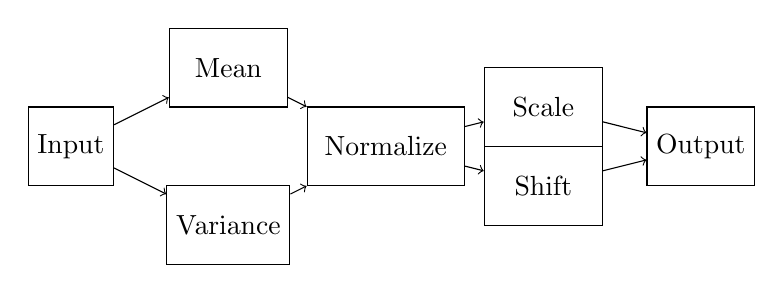
\begin{tikzpicture}
    % Draw input
    \node (input) at (0, 0) [draw, rectangle, minimum width=1cm, minimum height=1cm] {Input};

    % Draw BN layers
    \node (mean) at (2, 1) [draw, rectangle, minimum width=1.5cm, minimum height=1cm] {Mean};
    \node (variance) at (2, -1) [draw, rectangle, minimum width=1.5cm, minimum height=1cm] {Variance};

    \node (normalize) at (4, 0) [draw, rectangle, minimum width=2cm, minimum height=1cm] {Normalize};

    \node (scale) at (6, 0.5) [draw, rectangle, minimum width=1.5cm, minimum height=1cm] {Scale};
    \node (shift) at (6, -0.5) [draw, rectangle, minimum width=1.5cm, minimum height=1cm] {Shift};

    % Draw output
    \node (output) at (8, 0) [draw, rectangle, minimum width=1cm, minimum height=1cm] {Output};

    % Draw arrows
    \draw[->] (input) -- (mean);
    \draw[->] (input) -- (variance);
    \draw[->] (mean) -- (normalize);
    \draw[->] (variance) -- (normalize);
    \draw[->] (normalize) -- (scale);
    \draw[->] (normalize) -- (shift);
    \draw[->] (scale) -- (output);
    \draw[->] (shift) -- (output);
\end{tikzpicture}
\end{center}


















\section{Generative Adversarial Networks (GANs)}

\subsection{Original GAN Loss Functions}

\subsubsection{Discriminator Loss}
\begin{equation}
L_D = - \mathbb{E}_{\mathbf{x} \sim p_{\text{data}}} [\log D(\mathbf{x})] - \mathbb{E}_{\mathbf{z} \sim p_{\mathbf{z}}} [\log (1 - D(G(\mathbf{z})))]
\end{equation}

\subsubsection{Generator Loss}
\begin{equation}
L_G = - \mathbb{E}_{\mathbf{z} \sim p_{\mathbf{z}}} [\log D(G(\mathbf{z}))]
\end{equation}

\subsection{Non-Saturating GAN Loss}
\begin{equation}
L_G = \mathbb{E}_{\mathbf{z} \sim p_{\mathbf{z}}} [\log (1 - D(G(\mathbf{z})))]
\end{equation}

\subsection{Least Squares GAN (LSGAN)}

\subsubsection{Discriminator Loss}
\begin{equation}
L_D = \frac{1}{2} \mathbb{E}_{\mathbf{x} \sim p_{\text{data}}} [(D(\mathbf{x}) - 1)^2] + \frac{1}{2} \mathbb{E}_{\mathbf{z} \sim p_{\mathbf{z}}} [D(G(\mathbf{z}))^2]
\end{equation}

\subsubsection{Generator Loss}
\begin{equation}
L_G = \frac{1}{2} \mathbb{E}_{\mathbf{z} \sim p_{\mathbf{z}}} [(D(G(\mathbf{z})) - 1)^2]
\end{equation}

\subsection{Wasserstein GAN (WGAN)}

\subsubsection{Critic (Discriminator) Loss}
\begin{equation}
L_D = - \mathbb{E}_{\mathbf{x} \sim p_{\text{data}}} [D(\mathbf{x})] + \mathbb{E}_{\mathbf{z} \sim p_{\mathbf{z}}} [D(G(\mathbf{z}))]
\end{equation}

\subsubsection{Generator Loss}
\begin{equation}
L_G = - \mathbb{E}_{\mathbf{z} \sim p_{\mathbf{z}}} [D(G(\mathbf{z}))]
\end{equation}

\subsection{Wasserstein GAN with Gradient Penalty (WGAN-GP)}

\subsubsection{Critic (Discriminator) Loss with Gradient Penalty}
\begin{equation}
\begin{aligned}
L_D = &- \mathbb{E}_{\mathbf{x} \sim p_{\text{data}}} [D(\mathbf{x})] + \mathbb{E}_{\mathbf{z} \sim p_{\mathbf{z}}} [D(G(\mathbf{z}))] \\
&+ \lambda \mathbb{E}_{\hat{\mathbf{x}} \sim p_{\hat{\mathbf{x}}}} \left[ (|| \nabla_{\hat{\mathbf{x}}} D(\hat{\mathbf{x}}) ||_2 - 1)^2 \right]
\end{aligned}
\end{equation}

















\section{RNNs}

\begin{equation}
h_t = \text{ReLU}(W_h h_{t-1} + W_x x_t)
\end{equation}

\begin{equation}
\frac{\partial h_t}{\partial W_h} = \frac{\partial \text{A}(z_t)}{\partial z_t} \cdot \left( W_h \cdot \frac{\partial h_{t-1}}{\partial W_h} + h_{t-1} \right)
\end{equation}

\begin{equation}
\frac{\partial h_t}{\partial W_x} = \frac{\partial \text{A}(z_t)}{\partial z_t} \cdot \left( W_h \cdot \frac{\partial h_{t-1}}{\partial W_x} + x_t \right)
\end{equation}

\begin{equation}
\frac{\partial h_t}{\partial x_\tau} = \frac{\partial \text{A}(z_t)}{\partial z_t} \cdot \left( W_h \cdot \frac{\partial h_{t-1}}{\partial x_\tau} + W_x \cdot \delta_{\tau t} \right)
\end{equation}

\section{GRUs}

\begin{equation}
z_t = \sigma(W_z x_t + U_z h_{t-1})
\end{equation}

\begin{equation}
r_t = \sigma(W_r x_t + U_r h_{t-1})
\end{equation}

\begin{equation}
\tilde{h}_t = \text{tanh}(W_h x_t + U_h (r_t \odot h_{t-1}))
\end{equation}

\begin{equation}
h_t = (1 - z_t) \odot h_{t-1} + z_t \odot \tilde{h}_t
\end{equation}

\section{LSTMs}

\begin{equation}
i_t = \sigma(W_i x_t + U_i h_{t-1} + b_i)
\end{equation}

\begin{equation}
f_t = \sigma(W_f x_t + U_f h_{t-1} + b_f)
\end{equation}

\begin{equation}
o_t = \sigma(W_o x_t + U_o h_{t-1} + b_o)
\end{equation}

\begin{equation}
\tilde{C}_t = \text{tanh}(W_C x_t + U_C h_{t-1} + b_C)
\end{equation}

\begin{equation}
C_t = f_t \odot C_{t-1} + i_t \odot \tilde{C}_t
\end{equation}

\begin{equation}
h_t = o_t \odot \text{tanh}(C_t)
\end{equation}

\section*{Exploding and Vanishing Gradients in RNNs}

\subsection*{Recurrence Relation}

For a standard RNN, the hidden state \( h_t \) at time \( t \) is given by:
\begin{equation}
h_t = \phi(W_h h_{t-1} + W_x x_t)
\end{equation}
where \( \phi \) is the activation function, typically \( \tanh \) or \text{ReLU}. For simplicity, we consider \( \phi \) to be the identity function:
\begin{equation}
h_t = W_h h_{t-1} + W_x x_t
\end{equation}

\subsection*{Backpropagation Through Time (BPTT)}

During BPTT, the gradient of the loss \( L \) with respect to the weight matrix \( W_h \) is computed by unrolling the RNN through time:
\begin{equation}
\frac{\partial L}{\partial W_h} = \sum_{t=1}^T \frac{\partial L}{\partial h_t} \frac{\partial h_t}{\partial W_h}
\end{equation}

To understand the gradient flow, we need to look at the partial derivative of the hidden state with respect to the previous hidden state:
\begin{equation}
\frac{\partial h_t}{\partial h_{t-1}} = W_h
\end{equation}

So, the gradient with respect to \( h_{t-1} \) can be written as:
\begin{equation}
\frac{\partial L}{\partial h_{t-1}} = \frac{\partial L}{\partial h_t} \frac{\partial h_t}{\partial h_{t-1}} = \frac{\partial L}{\partial h_t} W_h
\end{equation}

By recursively applying this through time, we get:
\begin{equation}
\frac{\partial L}{\partial h_0} = \left( \prod_{t=1}^{T} W_h \right) \frac{\partial L}{\partial h_T}
\end{equation}

\subsection*{Eigenvalues and Gradient Behavior}

The behavior of the gradients as they propagate backward through time is governed by the eigenvalues of the weight matrix \( W_h \):

\subsubsection*{Exploding Gradients}
If the eigenvalues \( \lambda_i \) of \( W_h \) are greater than 1, the gradients will grow exponentially as they propagate backward through time:
\begin{equation}
\left| \frac{\partial L}{\partial h_0} \right| = \left| \left( \prod_{t=1}^{T} \lambda_i \right) \frac{\partial L}{\partial h_T} \right| = \left| \lambda_i^T \frac{\partial L}{\partial h_T} \right|
\end{equation}
Since \( |\lambda_i| > 1 \), \( |\lambda_i^T| \) increases exponentially with \( T \), causing the gradients to explode.

\subsubsection*{Vanishing Gradients}
If the eigenvalues \( \lambda_i \) of \( W_h \) are less than 1, the gradients will decay exponentially as they propagate backward through time:
\begin{equation}
\left| \frac{\partial L}{\partial h_0} \right| = \left| \left( \prod_{t=1}^{T} \lambda_i \right) \frac{\partial L}{\partial h_T} \right| = \left| \lambda_i^T \frac{\partial L}{\partial h_T} \right|
\end{equation}
Since \( |\lambda_i| < 1 \), \( |\lambda_i^T| \) decreases exponentially with \( T \), causing the gradients to vanish.

\subsection*{Mathematical Summary}

\subsubsection*{Exploding Gradients}
When \( |\lambda_i| > 1 \):
\begin{equation}
\left| \frac{\partial L}{\partial h_t} \right| = \left| \lambda_i^t \frac{\partial L}{\partial h_T} \right|
\end{equation}
As \( t \) increases, \( |\lambda_i^t| \) grows exponentially, leading to exploding gradients.

\subsubsection*{Vanishing Gradients}
When \( |\lambda_i| < 1 \):
\begin{equation}
\left| \frac{\partial L}{\partial h_t} \right| = \left| \lambda_i^t \frac{\partial L}{\partial h_T} \right|
\end{equation}
As \( t \) increases, \( |\lambda_i^t| \) decays exponentially, leading to vanishing gradients.

\end{document}